\chapter{Relevant Facts and Assumptions}

This chapter covers the relevant facts and assumptions that were made during the development of this project. It describes the customer base of Caruso and their needs. It also covers the topic of the development time on the side of Caruso.

% facts and assumptions that are not constraints or requirements. E. g. intresting information, delining the context.
There are a wide variety of customers that Caruso is looking to acquire. \autoref{caruso-customers} shows which of them are the most valuable customers. Carvis should mainly focus on those in the top right corner, as they are the best prepared and represent the highest yield opportunity.

\begin{figure}[ht]
  \centering
  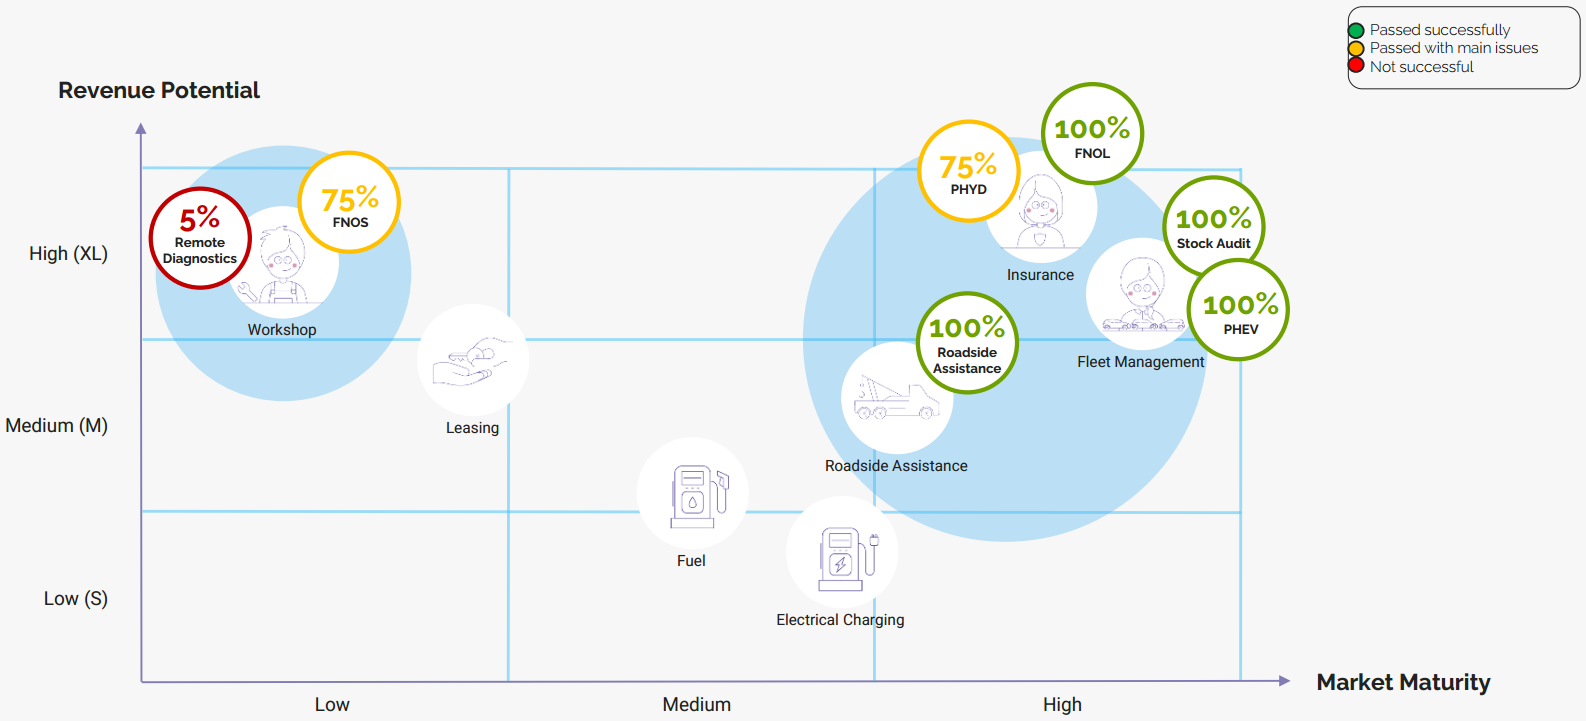
\includegraphics[width=\textwidth]{relevant_facts_and_assumptions/caruso-use-cases.png}
  \caption{Graph of different Caruso customers ordered by revenue potential and market maturity.}
  \label{caruso-customers}
\end{figure}

A possible conclusion to the aforementioned statement could be that only large companies are compelling customers, which is not the case. Large companies have a lot of resources to invest in innovative technologies, so the demand for a \gls{appetiser} is lower. On the other hand, medium-sized companies typically want to know what they are investing their money and time into before allocating resources. This is where Carvis helps to highlight areas where Caruso \glspl{data} can be used.

The goal of this project is to deliver a finished product that meets the needs of our \glspl{stakeholder}, including Caruso. We understand that Caruso may not want to invest additional development time of their team to make adjustments to the application. As such, a modular system is the best solution for this project.